

As discussed in Symbols chapter, there is a layer of the Geometron Hypercube devoted to 3d geometric actions in software(as opposed to machine control).  These actions are assigned the addresses between 0700 and 0777(base 8).  For each action, there is a two-dimensional Geometron symbol with addresses equal to the actions, but with a 1 before them, ranging from 01700 through 01777(base 8).  As with the rest of Geometron, we can edit a glyph which is made up of a sequence of geometric actions using an interface based on manipulating the symbols which represent those actions in a Web browser.

While it is possible to use the full grid of all 64 actions to create extremely complex three dimensional constructions, for the purpose of this work we restrict ourselves to a few basic actions.  As with all other parts of Geometron we use the fact that discrete motions along the available geometric directions combined with halving and doubling of the unit of movement is sufficient to move a cursor to any place in space.  We therefore have as our basic actions 6 discrete movements along three axes, the halving and doubling of the unit of motion, and the construction of a sphere and a cube, along with actions to select colors. 


\begin{figure}
	\centering
	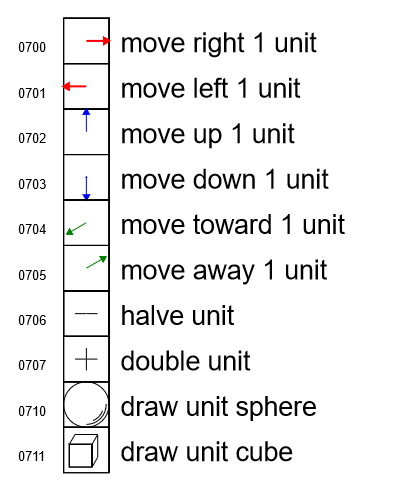
\includegraphics[width=3in]{figures/geometron3d/actions.png}
	\caption[actions3d]
	{Actions.  This is a minimalistic action set. More complex actions are added based on specialized applications.}
\end{figure}

The addresses in the Hypercube from 0600 through 0677 represent ``shapes'' in three dimensional Geometron, which also have two dimensional Geometron symbols in the range from 01600 to 01677.  These can be used to build up arbitrarily complex objects with layers of structural hierarchy.  As an example of how useful this is, we will show how we can build up a universal rectangular base on which to print symbols.  


\begin{figure}
	\centering
	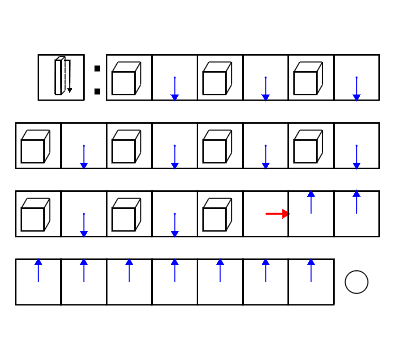
\includegraphics[width=3in]{figures/geometron3d/shapebuilding1.png}
	\caption[shapebuilding1]
	{A linear rectangular solid can be built up using a sequence of repeated cubes.  This 3d shape is then ready for use in more complex structures.}
\end{figure}

\begin{figure}
	\centering
	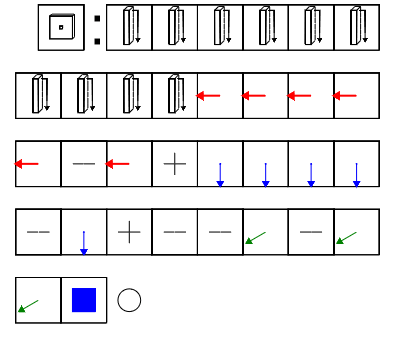
\includegraphics[width=3in]{figures/geometron3d/shapebuilding2.png}
	\caption[shapebuilding2]
	{Linear rectangular solids can be used to build up a flat rectangular plate shape.  The shape shown here builds this structure, then shrinks down to the size of a single pixel which will be used in the construction of 3d printed icons with the same bytecode as used in the rest of the system.}
\end{figure}


In Geometron we are always concerned with making useful files which can lead to either physical production or have some function in operating the overall system.  We also want to be able to replicate symbols created in other parts of the system in the three dimensional spaces we create using the software.  To see what is useful for this, we have to discuss some of the formats and tools available for three dimensional graphics in Web browsers and in everyday use.  

The most basic way to render three dimensional graphics, and the oldest on the Web is to use the current updated version of what used to be called VRML, or Virtual Reality Markup Language.  This was the original format back in the 1990's when people were first talking about a new way to exist on the Internet with ubiquitous virtual reality.  This new web never materialized.  Also, VRML was replaced by a newer more widely used format, called x3d, which is a subset of XML, just like HTML.

The most general three dimensional Geometron app is called voxel.html.  A ``voxel'' is the three dimensional extension of the idea of a ``pixel'', and this software can be used to quickly draw three dimensional objects in the browser using either softkeys or a special keyboard mapping specifically for 3d.  The way voxel.html works, much like most Geometron apps is that it edits in real time the value of a file stored in the Geometron server at data/glyph3d.txt.  This glyph is a string consisting of a sequence of base 8 numbers separated by commas as usual in Geometron.  Also, as usual, as we edit a glyph the text input with the glyph code is updated live.  We can always copy and paste any glyph from any instance of Geometron to any other. So if you are making a glyph in your local private server and send a private text message to another person with the text in the glyph input copied, they can paste that into the private server on their network and instantly replicate your glyph in their system.  The way the app voxel.html works is that it has a local function in the HTML code which acts on the Geometron Hypercube by manipulating global geometric variables x, y and z, and constructing shapes in an x3d object.  The specification of x3d contains basic geometry primitives such as cube and sphere, as well as transformations like translation and scale operations.

All of this work is carried out using the x3dom JavaScript library x3dom.js.  This is documented at www.x3dom.org.  This library allows for creation of x3d objects in an HTML file using DOM(Document Object Model) JavaScript commands.  As the JavaScript code alters the x3d object, however, it creates actual human readable code which can be copied into a separate x3d file.  This is done with the ``save'' button which copies the x3d code into another html file wrapped in a header and footer to make it render in a browser, called three.html.  Every time someone hits the ``save'' button the old version of three.html is destroyed and replaced with a new version with whatever the current status of the 3d object is in voxel.html.  The source code of three.html can be copy/pasted as a x3d object which can be embedded in any type of VR system which uses that format.  This can be used to create games and virtual reality or augmented reality applications based on Geometron.

Another method for creating 3d graphics in the Web is the use of WebGL, a cross-browser graphics framework, via the JavaScript library Three.js.  This fantastically powerful and well-documented library is another free open source library with publicly available CDNs for easy use. For more details see the home page of the project at threejs.org.  The Geometron app threejs.html opens the same glyph file edited by voxel.html and renders it using three.js.  This passive program serves two purposes. First of all, it implements the whole basic Geometron Hypercube using the three.js library, which can form a jumping off point for developers reading this to create more interesting applications such as games or other dynamic user interfaces.  But its more immediate utility is the three.js library's ability to export to the .stl format.  This format turns 3d surfaces into meshes of triangles, and is the universal language used by 3d printer software.  Thus the ability to export from a Geometron glyph to .stl allows us to 3d print objects we create in Geometron.  This adds yet another physical layer to the types of media which we can exchange using Geometron code.  When the page threejs.html loads it automatically saves another file called data/three.stl, which can be downloaded by right clicking on the link, and that .stl file can be shared with anyone with a 3d printer to print it out.  That .stl file can also be opened with a lot of 3d editing software and integrated into other projects, allowing us to make icons which other people can integrate into other physical designs for 3d printers or even CNC and/or injection molding.  Note that the .stl files can get very large, and above a certain size the Geometron software will fail to save, as there is a limit to the size we can pass via the POST command in PHP.  We leave this limit in place to keep the system working with modest sized files.  This limit often makes spheres problematic and we replace them with cubes when we want to 3d print.

The app shapes3d.html allows us to edit Geometron glyphs stored in addresses from 0600 through 0607 in the Geometron Hypercube using the same editor style as in voxel.html.  Up and down arrows cycle through the addresses.  As glyphs are edited in each address, the global value of the hypercube stored at data/hypercube.txt is edited in real time.  Each action sequence glyph in the range 0600 through 0607 has a corresponding symbol glyph made of 2d Geometron actions in the address range from 01600 through 01607.  These are edited in a similar manner to other Geometron Hypercube stacks using the app shapes3dsymbols.html, which is linked from shapes3d.html.  

As an example of using this method of building up actions to make shapes which are built up into more complex shapes, we will create a simple castle object.  This starts with constructing a single tower made up of cubes of decreasing size(see figure).  We can then repeat this turret and move repeatedly to build up a square wall to make a sort of castle, the Castle of Whimsy(see figures).  

\begin{figure}
	\centering
	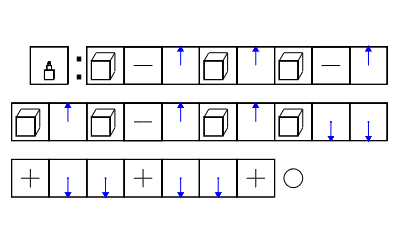
\includegraphics[width=3in]{figures/geometron3d/whimsycastleturret.png}
	\caption[whimsycastleturret]
	{Turret construction. Cubes of decreasing size make a whimsical turret.}
\end{figure}

\begin{figure}
	\centering
	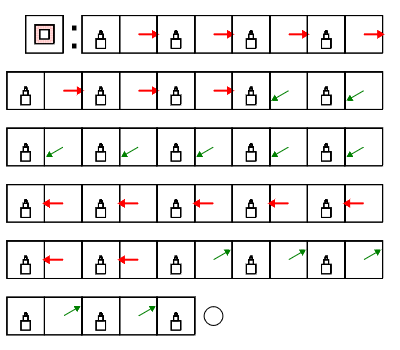
\includegraphics[width=3in]{figures/geometron3d/whimsycastlespelling.png}
	\caption[whimsycastlespelling]
	{Many turret glyphs can be called to build up a castle.}
\end{figure}

\begin{figure}
	\centering
	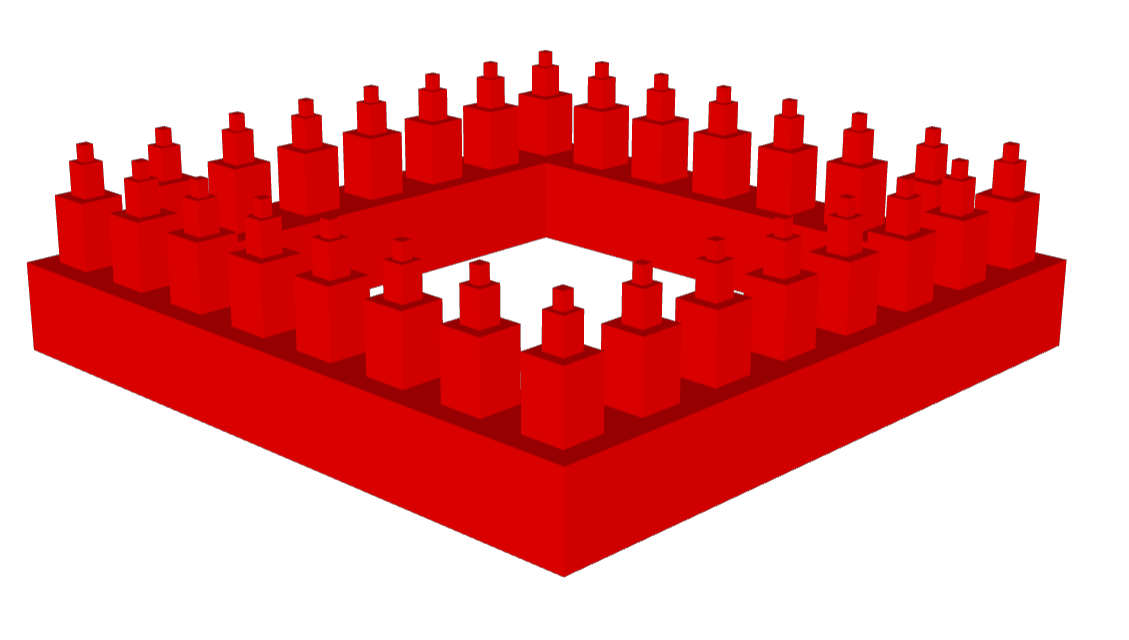
\includegraphics[width=3in]{figures/geometron3d/whimsycastle.png}
	\caption[whimsycastle]
	{The finished product: a whimsical castle object, ready to use in VR, AR, or to send to a 3d printer.}
\end{figure}


We will now explore how the system described above is combined with the overall power of Trash Robot and Geometron to build symbols which link to the rest of the system here.  The whole system of creating symbols for sharing in Trash Robot is based on pixel movements stored in addresses 0500 through 0507.  These elements as previously documented both draw pixels on a screen in a canvas element(or SVG) and also control the motors in any of a number of robotic systems which prints in any of various materials.  We now add yet another sequence of actions to these: movement with the drawing of a cube as a pixel(also known as a ``voxel'').  As with the robot control, We further add 3d geometry actions to the movement commands 0504 through 0507, so that we have the ability to move the 3d cursor around either with or without drawing a voxel.  If we combine this with creating a base tablet in the form of a large array of cubes in a plane, we can create either 3d web assets for VR, AR and other 3d web graphics and also can create 3d printable objects to share, all from the same robot code used in the rest of the Trash Robot system.  Just as we have an app for choosing an icon from the Trash Robot icon feed to print in the Trash Robot two and a half D printer, we have an app called icon3d.html which has a listing of all the Trash Robot icons, and when one is selected it loads up a 3d object with the icon printed in cubic voxels on the surface of a 8x8x1 rectangular solid.  As in voxel.html, clicking on the ``save'' button will  save the file to three.html, and loading the page threejs.html will resave the value of three.stl, overwriting the old version, for download and 3d printing.  This system means that we can freely share feeds of icon glyphs which can be physically shared by 3d printing in addition to all the other methods of sharing.  

3d printed parts can be used to stamp the symbol into soft objects, or used to make molds used to cast pourable objects with the icon in them.  Simple modification of the values of the hypercube to reverse the sign of the x direction can create a mirror image in the 3d object, which can be useful if we wish to create a stamp which when imprinted into soft objects directly prints the icon without having to create another negative.  Thus we can use 3d printing and basic Geometron operations to create copies of freely shared icons in any of a vast potential universe of materials both hard and soft.  We can store feeds of icons in Geometron Trash Robot code in globally accessible text files, and link to those text files on pages on Geometron server domains which we link to in URLs printed directly on 3d printed parts.  This makes the whole system self-replicating.  Someone can pass you a 3d printed part which has an icon on it which directs you to a domain name which hosts a site which links to a feed which has a list of icons all of which can be replicated in another 3d printer just by clicking on them.  This represents a decentralized network of free sharing of physical objects imprinted with icons which represent arbitrary things, to go along with all the other versions of this documented in other chapters.

\begin{figure}
	\centering
	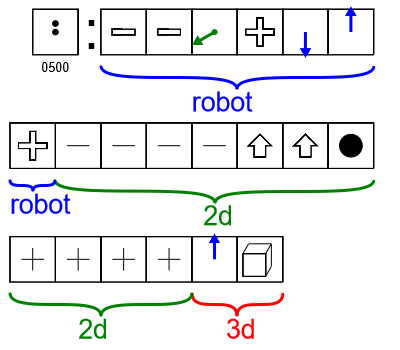
\includegraphics[width=3in]{figures/geometron3d/robot0500.png}
	\caption[robot0500]
	{Breakdown of how the glyphs in the pixel code for constructing icons are built up by accessing different layers of the Geometron Hypercube.  First we move the mechanical printing machine if there is one, then we create the little circle for the pixel on the screen if there is one, then create the cube pixel in the 3d web graphics object if there is one.  Any parts which act on something that doesn't exist are ignored by the GVM, but the GVM abstraction allows one unified structure to describe behavior in all of these layers.}
\end{figure}

\begin{figure}
	\centering
	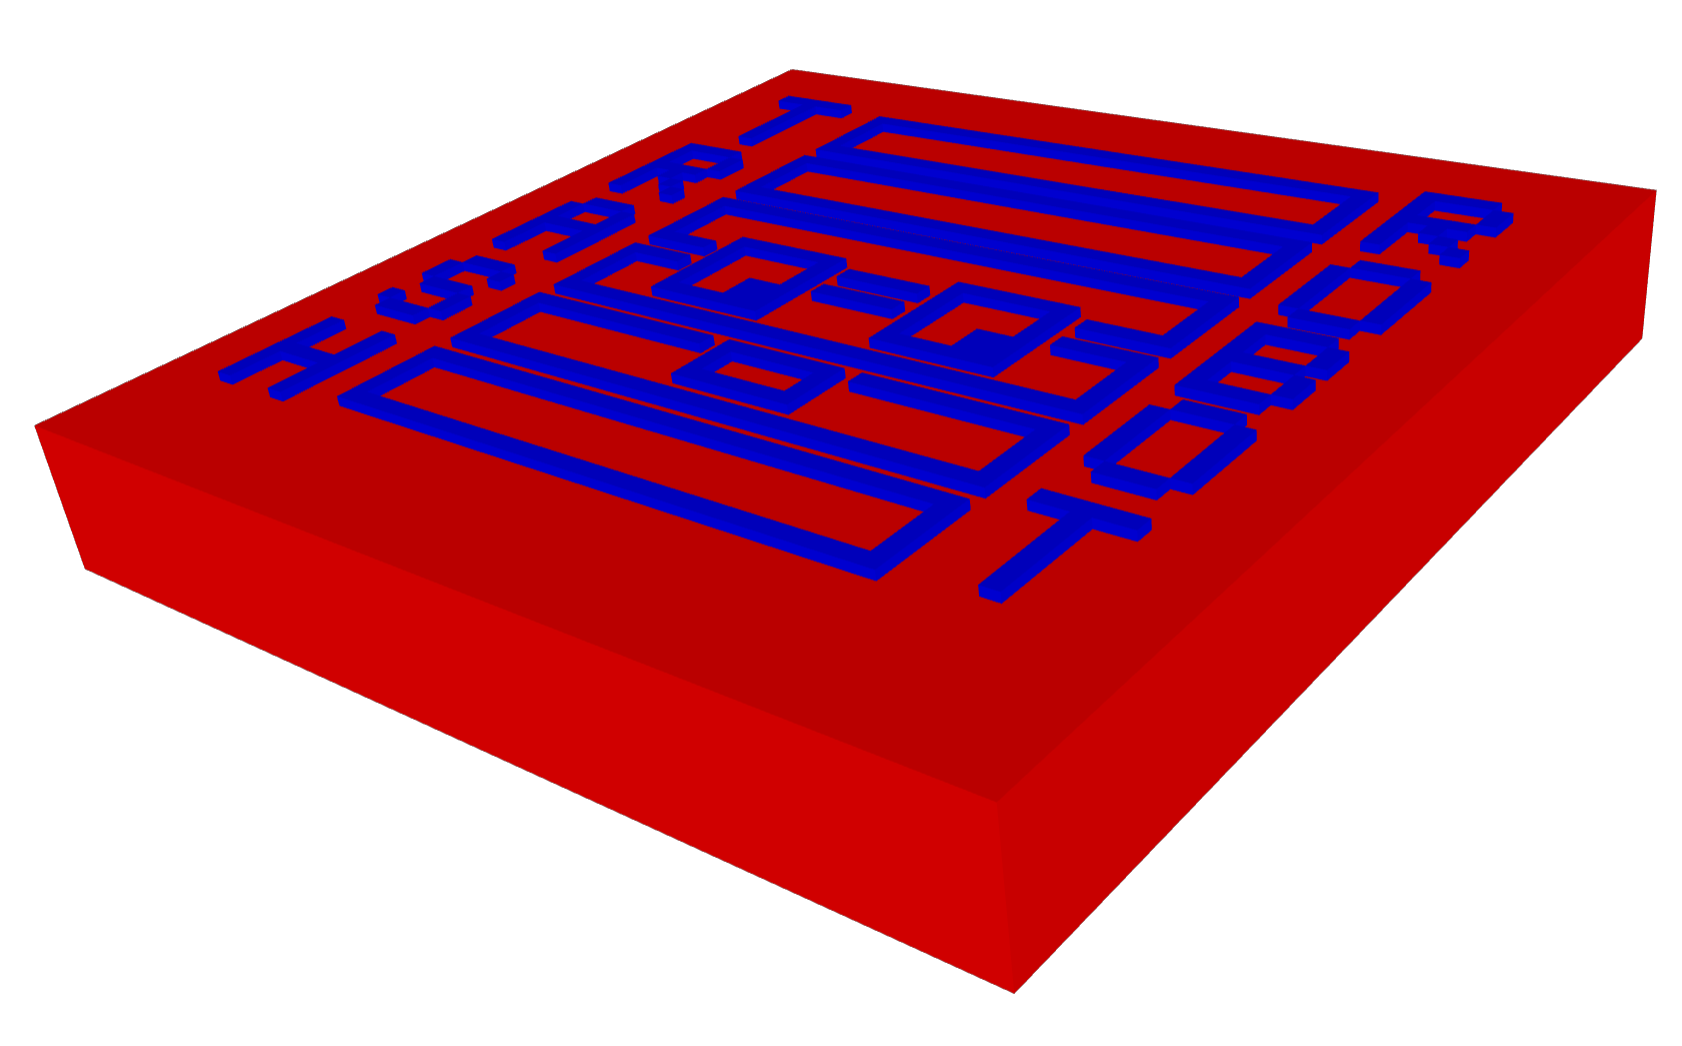
\includegraphics[width=3in]{figures/geometron3d/trashrobot3d.png}
	\caption[trashrobot3d]
	{An icon 3d object.  This is from a 3d web file, but can be converted into an .stl file to print on a 3d printer exactly as shown, and then it can be replicated by using it as a stamp to create molds which are used to make more copies.}
\end{figure}

\subsection{Rotations and Higher Dimensions}

As with every part of Geoemetron, we are only scratching the surface in this work of what can be done with these methods as we add actions to the Geometron Hypercube.  Of the available 64 actions in the Hypercube reserved for 3d geometric actions we have so far only used 18. Any type of discrete geometric action can be added.  In particular, rotations of rigid bodies is a deep field of mathematics which we have so far ignored.  So far we have only moved our geometric axes around along the x, y and z axes or scaled them all together.  We can add non-uniform scaling to make a much wider range of objects, and discrete rotations to create different orientations of objects.  We can also add a larger range of geometric primitives, such as cylinders, cones, and other custom, manually-constructed polyhedra.  

Discrete rotations can be a huge enabler of applications for Geometron.  By constructing spheres, moving along a radius vector, rotating, and moving, we can build up three dimensional models of molecules.  These molecules can then be simulated by recasting problems of how they fold in terms of angular rotations of the Geometron glyph used to construct them.  Sequences of chained discrete rotations can also be used to describe state vectors in the Hilbert space spanned by the qubits in a quantum processor.  An alternative way to think about quantum computing can therefore be constructed in which instead of programming bit states, we use Geometron to express states in terms entirely of rotation angles, and all gate control pulses can then be thought of as further discrete rotation operations.  If we map both states and dynamic operations in a quantum computer to Geometron glyphs, and also map problems of quantum chemistry(e.g. protein folding) into the same language, is seems at least plausible that such mapping could yield useful results in attempting to solve protein folding problems using the so-called NISQ(Noisy Intermediate Scale Quantum) systems which are presently available.  Also direct mapping between geometric operations in graphics displayed in a web browser and states or operations on a quantum processor admits the possibility of a very simple and powerful real time user interface for development of quantum algorithms, again on existing NISQ devices.  Such software could be easily created on top of the software frameworks currently under development by several parties. While this author believes quantum computing to be a complete waste of time which will never work, I find it amusing to pose this potential application in case someone wants to try it out, at least to make weird art on a quantum processor.  

\begin{figure}
	\centering
	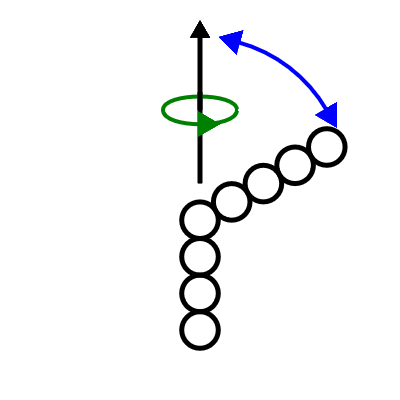
\includegraphics[width=4in]{figures/geometron3d/angles.png}
	\caption[angles]
	{This shows how a sequence of objects can be constructed with each object being a discrete distance along an axis of specified altitude and azimuth.  These angles can be manipulated with discrete rotations combined with step angle manipulations, just like the ones used in two dimensional Geometron constructions.}
\end{figure}

